\lstdefinestyle{MethodenListe}{
    language   = Python,
    numbers    = none,
    belowskip  = 0.25em,
    basicstyle = \tt\small
}

\lstdefinestyle{MethodenListeKlein}{
    language   = Python,
    numbers    = none,
    belowskip  = 0.25em,
    basicstyle = \tt\footnotesize
}

%-------------------------------------------------------------------------------
\section{Einführung in das Semester}
%-------------------------------------------------------------------------------

%%% Folie
\begin{frame}{Kompetenzziele der Vorlesung}
    \begin{itemize}
        \item \textbf{Fachkompetenz:} Die Studierenden kennen den technischen Aufbau typischer
        Devices/Embedded Systems im Kontext der Internet of Things. Sie sind in der Lage,
        entsprechende Devices für einen gegebenen Einsatzzweck auszuwählen und zu programmieren.
        \medskip

        \item \textbf{Methodenkompetenz:} Die Studierenden sind in der Lage bei der Programmierung
        von IoT-Geräten systematisch und methodisch vorzugehen.
        \medskip

        \item \textbf{Personale und soziale Kompetenz:} Die Studierenden verstehen die Herausforderungen
        des IoT für Unternehmen, Politik und Gesellschaft und sind in der Lage, diese kompetent zu diskutieren.
        \medskip

        \item \textbf{Übergreifende Handlungskompetenz:} Die Studierenden können reale betriebliche
        Problemstellungen im Kontext von IoT analysieren, Konzepte entwerfen und IoT-fähige Geräte
        programmieren und im Unternehmenskontext integrieren.
        \medskip
    \end{itemize}
\end{frame}

{
\footnotesize
%%% Folie
\begin{frame}{Inhalte der Vorlesung}
        \begin{columns}
            \begin{column}[T]{.5\textwidth}
                \begin{block}{3. Semester}
                    \medskip
                    \textbf{Prüfungsform:} Klausur
                    \medskip

                    \begin{enumerate}
                        \item Grundlagen des Internet of Things
                        \item Hardwaredesign für IoT-Anwendungen
                        \item \textcolor{gray}{Übungsstunde}
                        \item \textcolor{gray}{Übungsstunde}
                        \item Einführung in Python
                        \item IoT-Entwicklung mit Python
                        \item \textcolor{gray}{Übungsstunde}
                        \item \textcolor{gray}{Übungsstunde}
                        \item \textcolor{gray}{Klausurvorbereitung}
                    \end{enumerate}
                \end{block}
            \end{column}
            \begin{column}[T]{.5\textwidth}
                \begin{block}{4. Semester}
                    \medskip
                    \textbf{Prüfungsform:} Assignment
                    \medskip

                    \begin{enumerate}
                        \item Nutzung analoger und digitaler Bauteile
                        \item Python-Architekturmuster für IoT-Devices
                        \item Datenaustausch und Systemintegration
                        \item Linux-Konfiguration und Deployment
                        \item \textcolor{gray}{Assignment}
                        \item \textcolor{gray}{Assignment}
                        \item \textcolor{gray}{Assignment}
                        \item \textcolor{gray}{Assignment}
                        \item \textcolor{gray}{Assignment}
                    \end{enumerate}
                \end{block}
            \end{column}
        \end{columns}
\end{frame}
}

%%% Folie
{
\setbeamertemplate{background canvas}{
    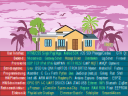
\includegraphics[height=\paperheight, width=\paperwidth]{1-grundlagen/img/themengebiete4}
}

\begin{frame}[plain]
\end{frame}
}

%%% Folie
\begin{frame}{Beispiel einer typischen IoT-Architektur}
    \begin{columns}
        \column{\dimexpr\paperwidth-10pt}
        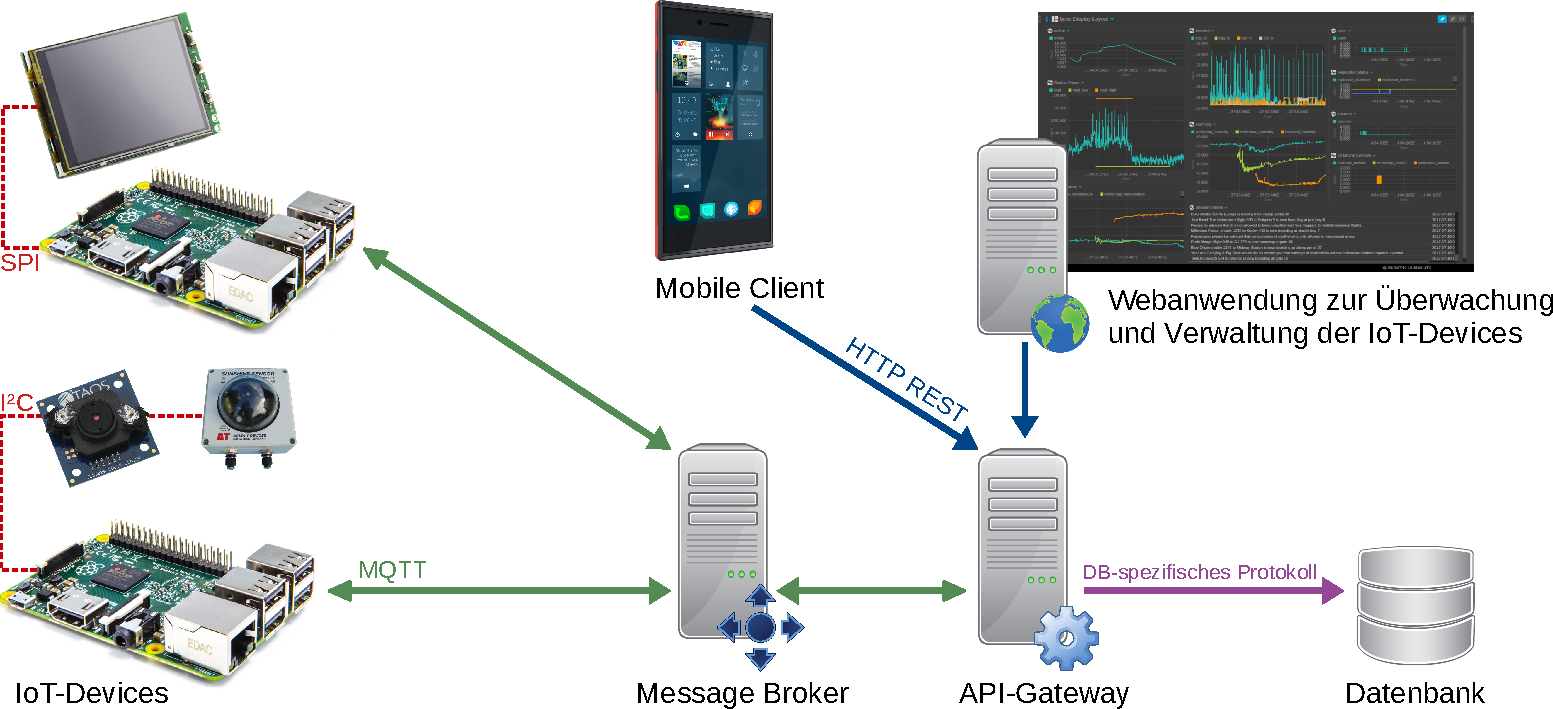
\includegraphics[width=\textwidth]{1-grundlagen/img/architektur_beispiel}
    \end{columns}
\end{frame}

%%% Folie
{
\small

\begin{frame}{Inhalt der Assignment-Prüfung}
    \begin{columns}[onlytextwidth]
        \column[t]{.45\textwidth}
        \begin{block}{Kreativaufgabe}
            \medskip
            \parbox{\linewidth}{
                Ausarbeitung eines Hard- und Softwareentwurfs zu einem \textbf{selbst gewählten IoT-Anwendungsfall}.
                \medskip

                Muss die wesentlichen Theorieinhalte beider Semester abdecken.
                \medskip

                Jedoch keinen Quellcode, keine Details und keine praktische Umsetzung. Nur das Konzept.
            }
        \end{block}

        \column[t]{.45\textwidth}
        \begin{block}{Programmieraufgabe}
            \medskip
            \parbox{\linewidth}{
                Praktische Umsetzung eines \textbf{vorgegebenen IoT-Anwendungsfalls}.
                \medskip

                Muss gegen vorgegebene Schnittstellen zum Mocken der Hardwareelemente
                programmiert werden.
                \medskip

                Bewertet werden die Qualität des Quellcodes und die Erfüllung der von
                uns vorgegebenen Unit Tests.
            }
        \end{block}
    \end{columns}

    \bigskip
    \bigskip
    {
        \normalsize
        Die Aufgabenstellung wird bis zum Ende des Theorieblocks bereitgestellt.
    }
\end{frame}
}

%%% Folie
{
\small
\setlength{\fboxsep}{0pt}

\begin{frame}{Literaturempfehlungen}
    \begin{columns}
        \column[b]{.25\textwidth}
        \fbox{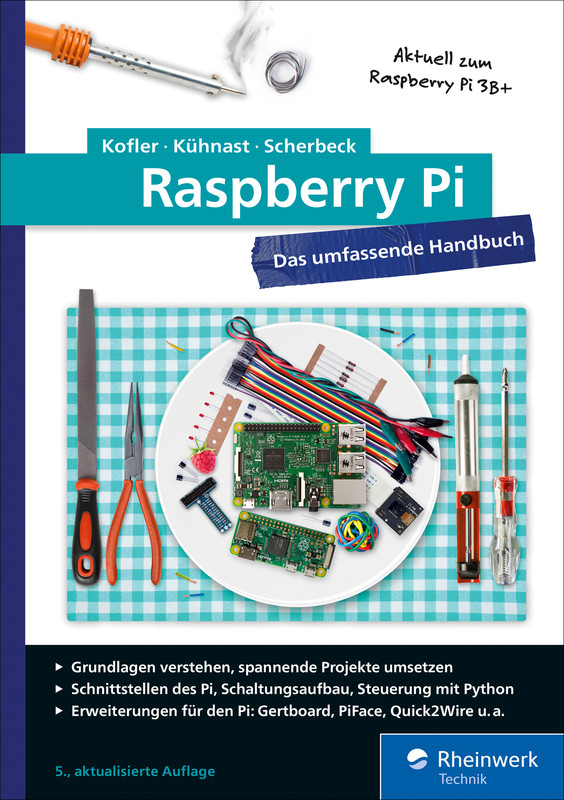
\includegraphics[height=3.8cm]{5-hardwarenutzung/img/buch_raspberrypi}}

        \column[b]{.25\textwidth}
        \fbox{
\includegraphics[height=3.8cm]{5-hardwarenutzung/img/buch_mqtt_essentials}}

        \column[b]{.25\textwidth}
        \fbox{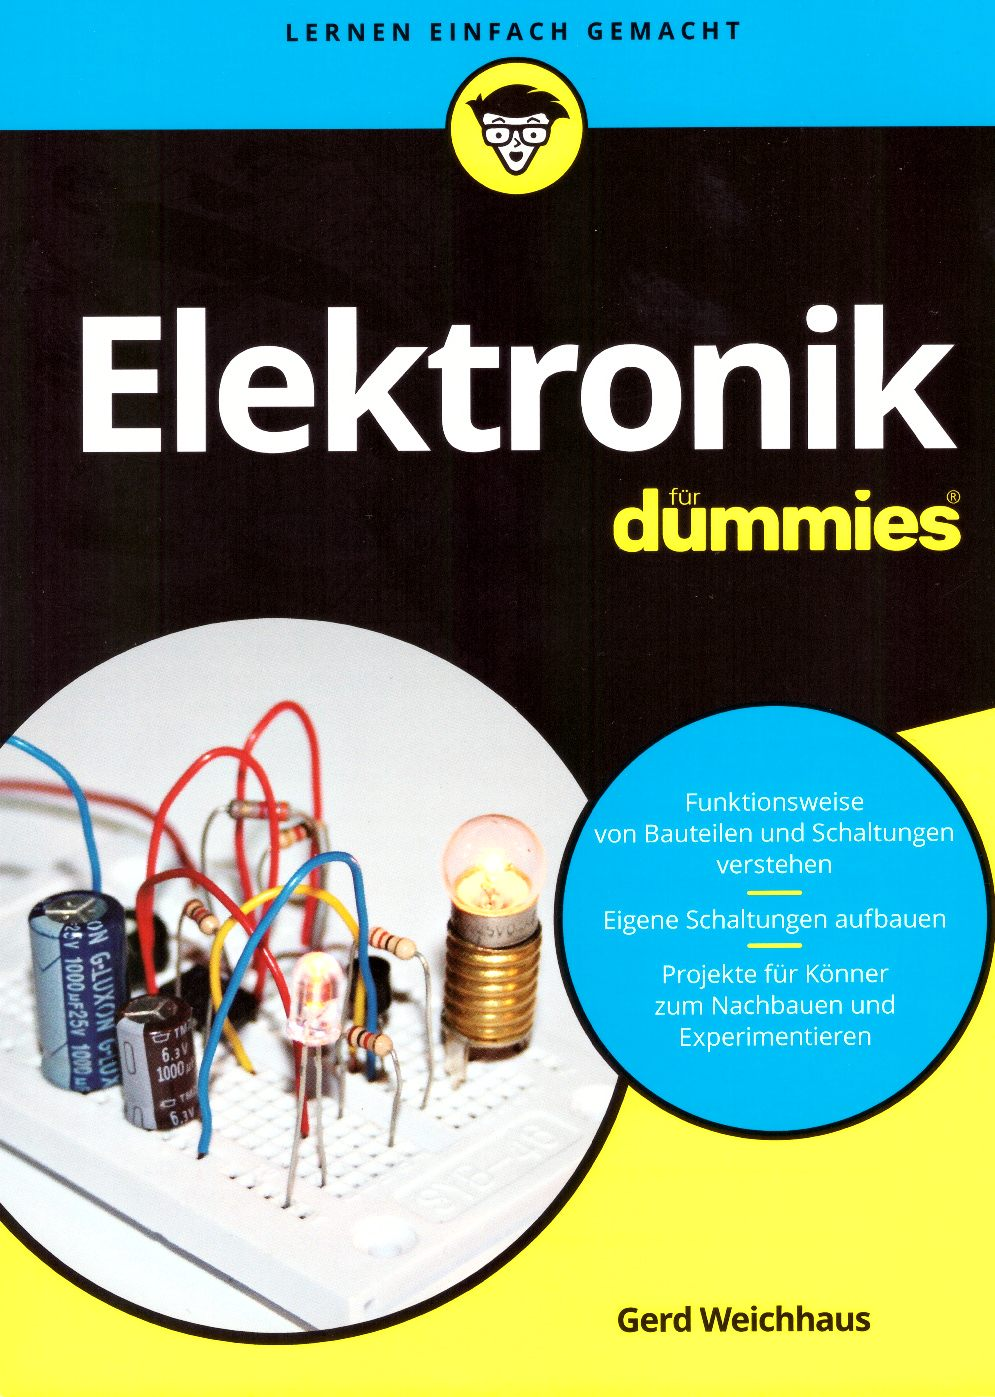
\includegraphics[height=3.8cm]{5-hardwarenutzung/img/buch_elektronik_dummies}}

        \column[b]{.25\textwidth}
        \fbox{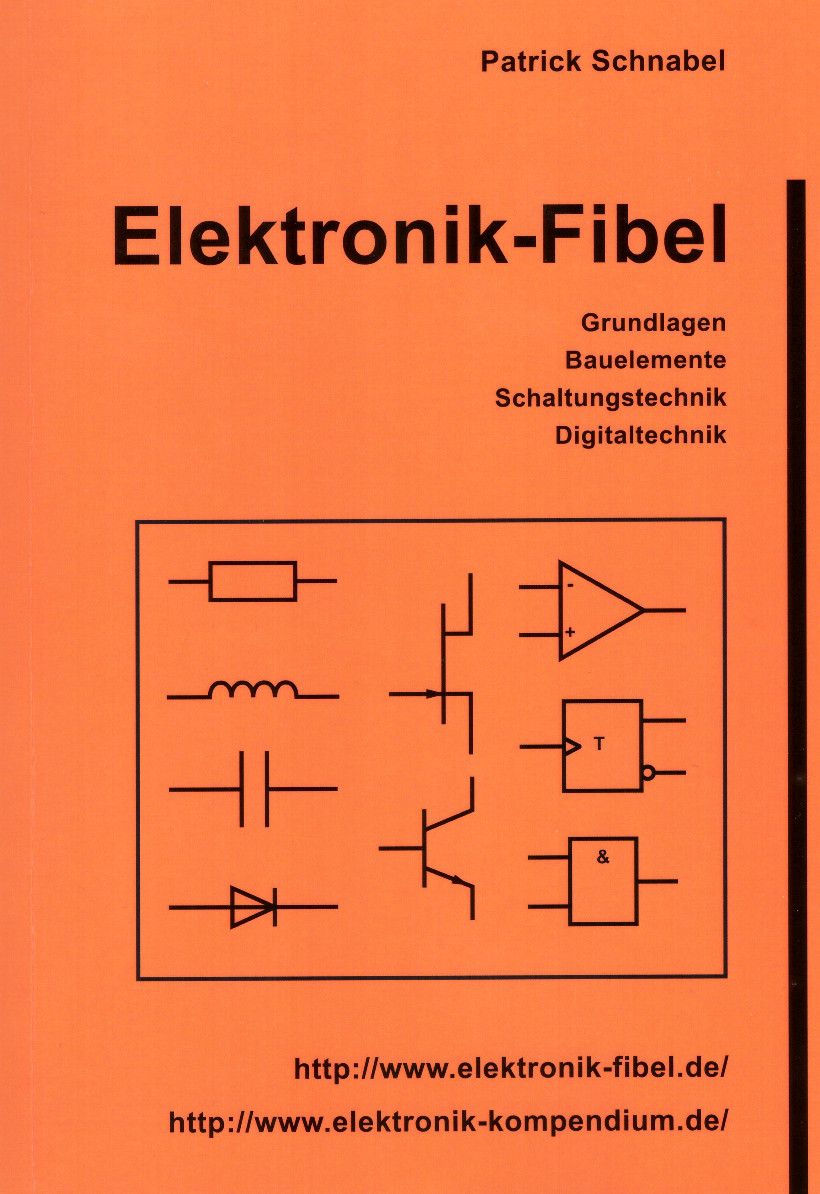
\includegraphics[height=3.8cm]{5-hardwarenutzung/img/buch_elektronik_fibel}}
    \end{columns}

    \vskip 0.6cm

    \begin{columns}
        \column[T]{.5\textwidth}
        \textbf{Raspberry Pi: Das umfassende Handbuch für Maker und Tekkies} \\ Rheinwerk Verlag, 2018

        \column[T]{.5\textwidth}
        \textbf{MQTT Essentials: \\ A Lightweight IoT Protocol} \\ Packt>, 2017
    \end{columns}

    \vskip 0.6cm

    \begin{columns}
        \column[T]{.5\textwidth}
        \textbf{Elektronik für Dummies} \\ Wiley-VCH Verlag, 2018

        \column[T]{.5\textwidth}
        \textbf{Elektronik-Fibel} \\ Patrick Schnabel, 2017
    \end{columns}
\end{frame}
}

%-------------------------------------------------------------------------------
\section{Ziel der heutigen Vorlesung}
%-------------------------------------------------------------------------------

%%% Folie
{
\footnotesize
\setlength{\leftmargini}{1.2em}

\begin{frame}{Typischer Systemaufbau eingebetteter Systeme}
    \begin{columns}
        \column{\dimexpr\paperwidth}

        \only<beamer:1|handout:0>{
            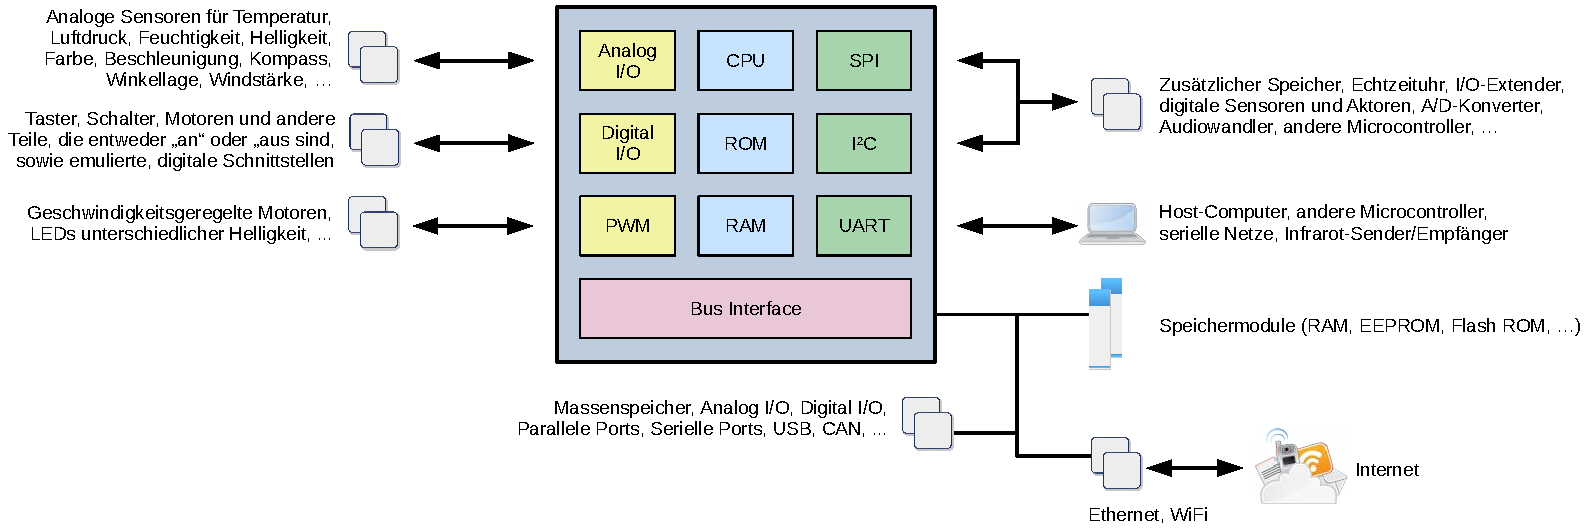
\includegraphics[width=\paperwidth]{5-hardwarenutzung/img/mc_aufbau1}
        }

        \only<beamer:2|handout:1>{
            \transdissolve
            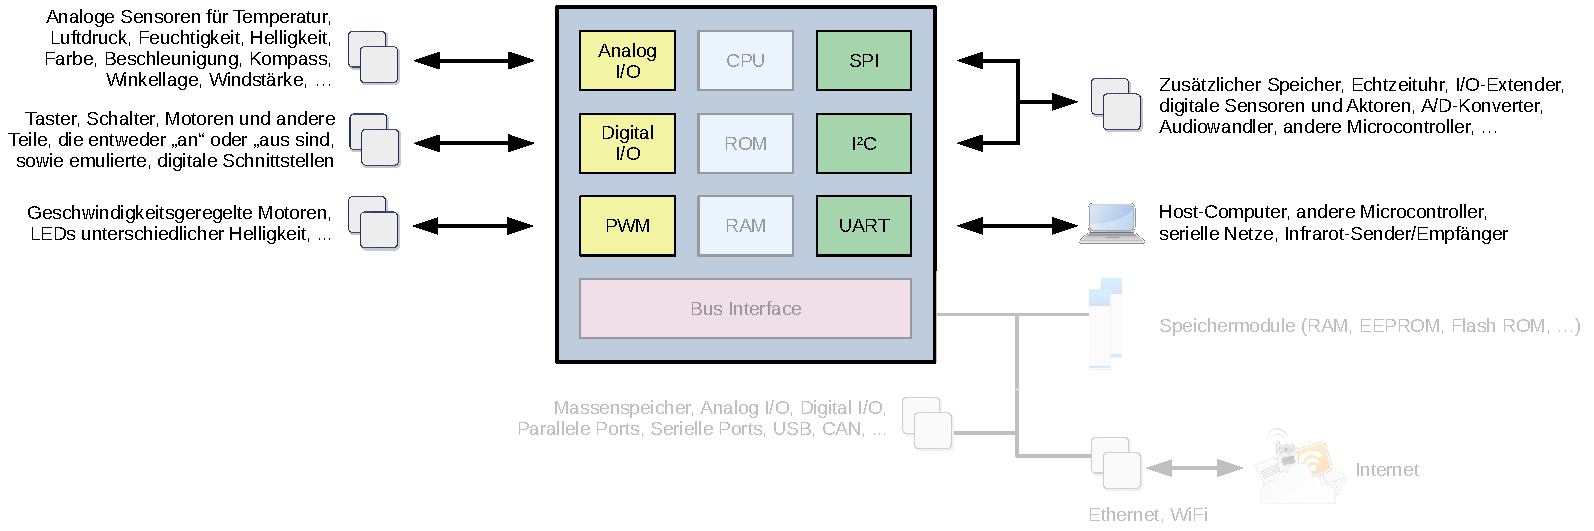
\includegraphics[width=\paperwidth]{5-hardwarenutzung/img/mc_aufbau2}
        }
    \end{columns}

    \medskip

    \begin{columns}
        \begin{column}[T]{.3\textwidth}
            \textbf{Raspberry Pi}
            \begin{itemize}
                \item Binäre Ein-/Ausgänge
                \item PWM-Ausgänge
                \item Serielle Ein-/Ausgänge
                \item<2> \textcolor{darkred}{Kein Analog I/O}
                \item<2> \textcolor{darkred}{Keine Bus Interface!}
            \end{itemize}
        \end{column}
        \begin{column}[T]{.3\textwidth}
            \textbf{Letztes Semester}
            \begin{itemize}
                \item Binäre Ein-/Ausgänge
                \item PWM-Ausgänge
                \item DHT11 via 1-Wire
                \item Programmierung in Python
            \end{itemize}
        \end{column}
        \begin{column}[T]{.3\textwidth}
            \textbf{Dieses Semester}
            \begin{itemize}
                \item Analog-Digital-Konverter
                \item Serielle Sensoren/Aktoren
                \item Serielle Kommunikation mit anderen µControllern
                \item Programmierung in Python
            \end{itemize}
        \end{column}
    \end{columns}
\end{frame}
}

%%% Folie
{
\scriptsize

\begin{frame}{Inhalt unseres Sensorkits}
    \begin{columns}[onlytextwidth]
        \column[T]{.3\textwidth}
        \textbf{Analoge Schnittstelle} \\
        KY-003: Hall Magnetfeldsensor \\
        KY-006: Passiver Piezo-Buzzer \\
        KY-009: RGB-LED \\
        KY-011: Rot/Grün-LED \\
        KY-012: Aktiver Piezo-Buzzer \\
        KY-013: Temperatursensor \\
        KY-016: RGB-LED \\
        KY-018: Fotowiderstand \\
        KY-023: XY-Joystick \\
        KY-024: Magnetic Hall-Sensor \\
        KY-025: Reedkontakt \\
        KY-026: Flammensensor \\
        KY-028: Thermistor \\
        KY-029: Rot/Grün-LED \\
        KY-034: 7-Farben LED \\
        KY-035: Bihor Magnetsensor \\
        KY-036: Metall-Touchsensor \\
        KY-037: Mikrofon Soundsensor \\
        KY-038: Mikrofon Soundsensor \\
        KY-039: Herzschlagsensor \\
        KY-040: Kodierter Drehschalter \\
        KY-050: Ultraschallabstand \\

        \column[T]{.3\textwidth}
        \textbf{Binäre An/Aus-Schnittstelle} \\
        KY-002: Erschütterungsschalter \\
        KY-003: Hall Magnetfeldsensor \\
        KY-004: Taster \\
        KY-010: Lichtschranke \\
        KY-012: Aktiver Piezo-Buzzer \\
        KY-017: Neigungsschalter \\
        KY-019: 5V Relais \\
        KY-020: Neigungsschalter \\
        KY-021: Mini Magnet-Reedkontakt \\
        KY-024: Magnetic Hall-Sensor \\
        KY-025: Reedkontakt \\
        KY-026: Flammensensor \\
        KY-027: Magic Light Cup \\
        KY-028: Thermistor \\
        KY-031: Klopfsensor \\
        KY-032: Hindernisdetektor \\
        KY-033: Trackingsensor \\
        KY-036: Metall-Touchsensor \\
        KY-037: Mikrofon Soundsensor \\
        KY-038: Mikrofon Soundsensor \\

        \column[T]{.3\textwidth}
        \textbf{Serielle Schnittstelle} \\
        KY-001: DS18B20 Temperatur \\
        KY-015: DHT11 Temp./Feuchtig. \\
        KY-052: BMP280 Druck \\
        KY-053: Analog/Digital Konverter \\
    \end{columns}

    \bigskip
    {
        \footnotesize
        Online-Dokumentation: \\
        \url{http://sensorkit.joy-it.net/index.php?title=Hauptseite}
    }
\end{frame}
}

%%% Folie
\begin{frame}{Lernziele}
    \begin{block}{Wiederholung}
        \begin{itemize}
            \item Breadboards zum Aufbau einfacher Schaltungen nutzen können
            \item Binäre Bauteile via GPIO mit dem Pi verbinden können
            \item Via GPIO angebundene Bauteile in Python nutzen können
        \end{itemize}
    \end{block}

    \begin{block}{Neue Inhalte}
        \begin{itemize}
            \item Funktionsweise serieller Schnittstellen erklären können
            \item Synchrone und asynchrone, serielle Schnittstellen abgrenzen können
            \item Digitale Bauteile via SPI, I²C mit dem Pi verbinden können
            \item Analoge Bauteile via A/D-Konverter mit dem Pi verbinden können
            \item Seriell angebundene Bauteile in Python nutzen können
        \end{itemize}
    \end{block}
\end{frame}

%-------------------------------------------------------------------------------
\section{Nutzung binärer Bauteile}
%-------------------------------------------------------------------------------

%%% Folie
{
\small
\setlength{\leftmargini}{1.2em}

\begin{frame}[allowframebreaks]{Fallbeispiel: Hindernisdetektor}
    \begin{columns}[onlytextwidth]
        \column{.49\textwidth}
        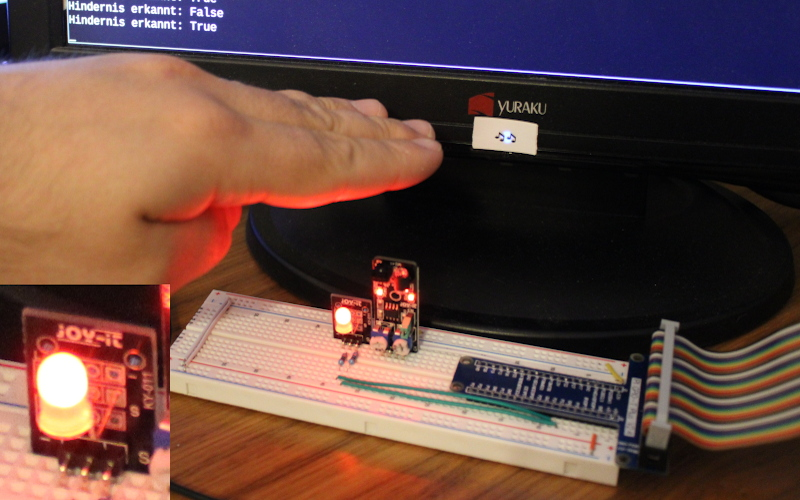
\includegraphics[width=\textwidth]{5-hardwarenutzung/img/hindernisdetektor-foto2}

        \column{.49\textwidth}
        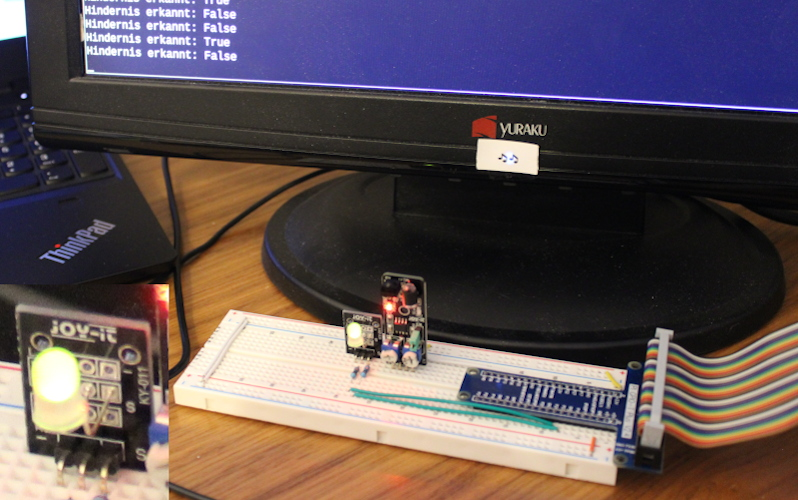
\includegraphics[width=\textwidth]{5-hardwarenutzung/img/hindernisdetektor-foto1}
    \end{columns}

    \bigskip
    Erkennung von Hindernissen mit dem KY-032 Hindernisdetektor und der KY-011
    2-Farb LED. Wird ein Hindernis erkannt, leuchtet die LED rot, andernfalls grün.

    \bigskip
    \begin{block}{Hardwareskizze}
        \smallskip
        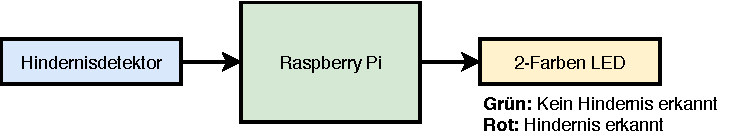
\includegraphics[width=\textwidth]{5-hardwarenutzung/img/hindernisdetektor-skizze}
    \end{block}

    \framebreak
    \begin{block}{Schaltplan}
        \smallskip
        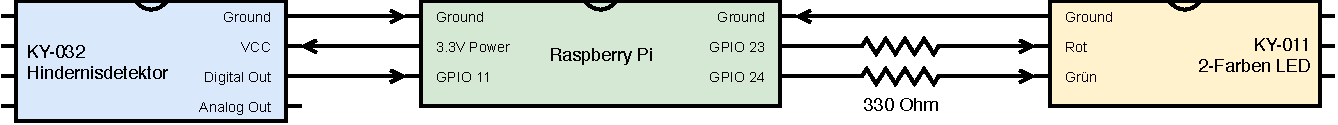
\includegraphics[width=\textwidth]{5-hardwarenutzung/img/hindernisdetektor-schaltplan}
        {
            \scriptsize
            Pfeile nur zur Verdeutlichung der Stromkreise. Normalerweise besitzt
            ein Schaltplan keine Pfeilenden.
        }
    \end{block}

    \bigskip

    \begin{block}{Hardwareaufbau}
        \smallskip
        \begin{columns}[onlytextwidth]
            \column[T]{.49\textwidth}
            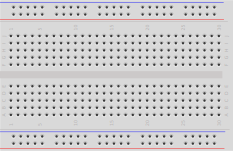
\includegraphics[width=\textwidth]{5-hardwarenutzung/img/breadboard1_bb}

            \column[T]{.49\textwidth}
            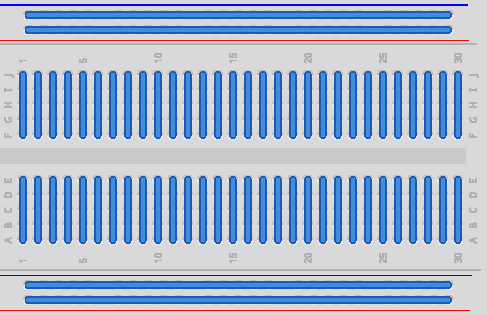
\includegraphics[width=\textwidth]{5-hardwarenutzung/img/breadboard2_bb}
        \end{columns}

        \smallskip
        {
            \scriptsize
            Die Linien auf der rechten Seite zeigen, wie die Kontakte des Breadboards
            miteinander verbunden sind.
        }
    \end{block}

    \framebreak
    \begin{columns}
        \column{.65\textwidth}
        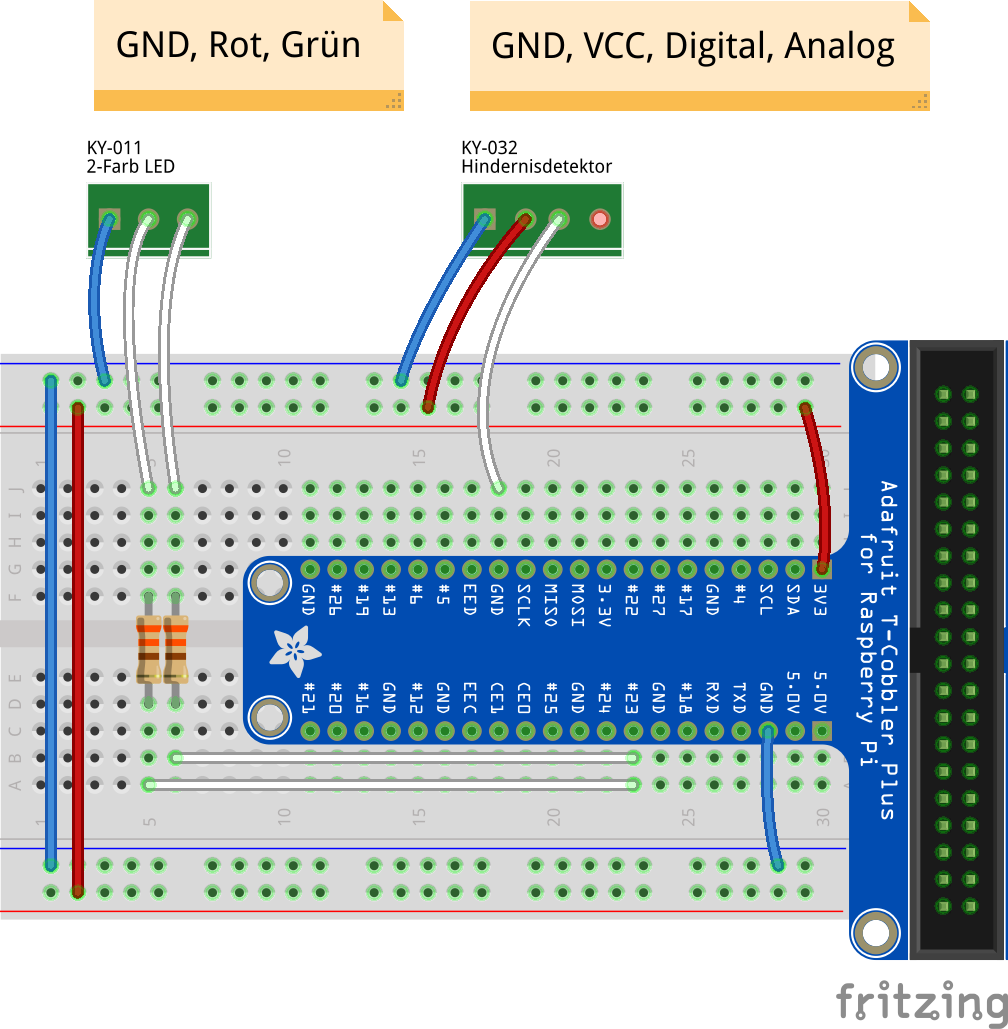
\includegraphics[width=\textwidth]{5-hardwarenutzung/img/hindernisdetektor_bb}

        \column{.35\textwidth}
        \begin{block}{Variationen}
            \medskip
            Nutzung anderer Sensoren

            {
                \footnotesize
                \begin{itemize}
                    \item Lichtschranke
                    \item Magnetkontakt
                    \item Berührungssensor
                    \item Schließkontakt
                    \item Neigungsschalter
                    \item \ldots
                \end{itemize}
            }

            \medskip
            Schalten größerer Lasten mit einem Transistor oder Relais

            {
                \footnotesize
                \begin{itemize}
                    \item Warnlampe einschalten
                    \item Durchgangstür öffnen
                    \item Förderband starten
                    \item \ldots
                \end{itemize}
            }
        \end{block}
    \end{columns}
\end{frame}
}

%%% Folie
{
\small
\setlength{\leftmargini}{1.2em}

\begin{frame}{Fallbeispiel: Servomotor}
    \begin{columns}[onlytextwidth]
        \column{.49\textwidth}
        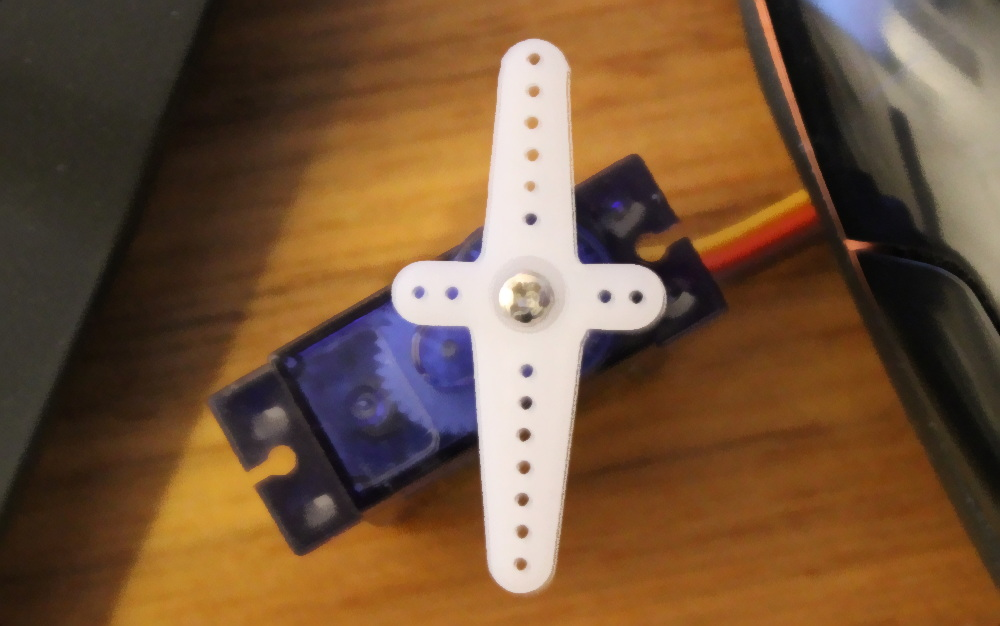
\includegraphics[width=\textwidth]{5-hardwarenutzung/img/servomotor-foto1}

        \column{.49\textwidth}
        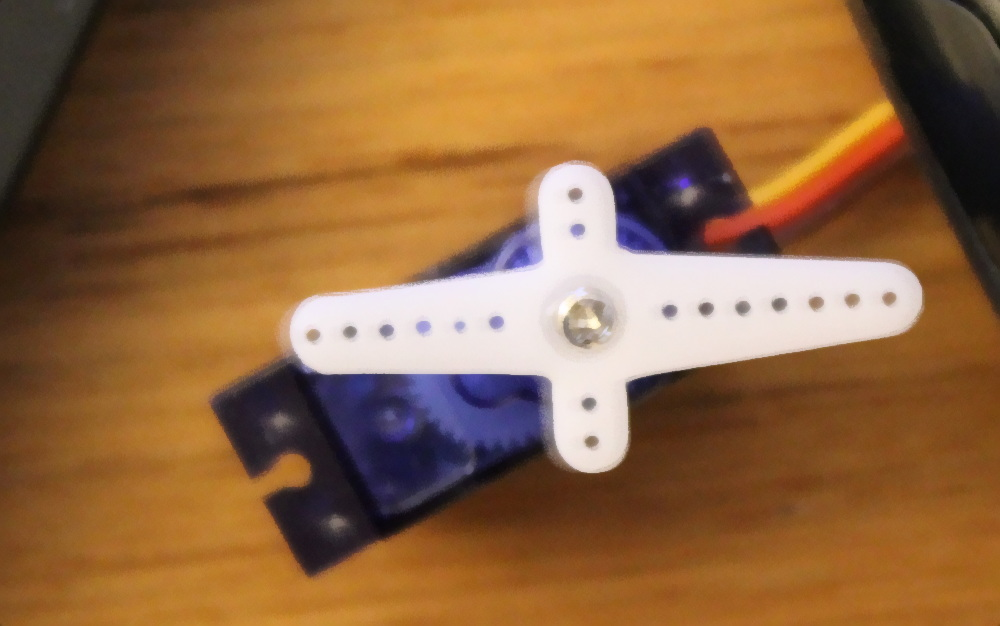
\includegraphics[width=\textwidth]{5-hardwarenutzung/img/servomotor-foto2}
    \end{columns}

    \bigskip
    Steuerung eines Servomotors mit Pulsweitenmodulation. Die Länge des Lastzyklus
    bestimmt die Position:

    {
        \footnotesize
        \smallskip
        \begin{itemize}
            \item \textbf{Ganz links:} 1\,ms Puls bei 50\,Hz Frequenz
            \item \textbf{Ganz rechts:} 2\,ms Puls bei 50\,Hz Frequenz
            \item \textbf{Andere:} Jeder Wert dazwischen
        \end{itemize}
    }

    \begin{columns}[onlytextwidth]
        \column[T]{.3\textwidth}
        \begin{block}{Hardwareskizze}
            \smallskip
            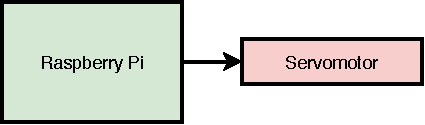
\includegraphics[width=\textwidth]{5-hardwarenutzung/img/servomotor-skizze}
        \end{block}

        \column[T]{.59\textwidth}
        \begin{block}{Schaltplan}
            \smallskip
            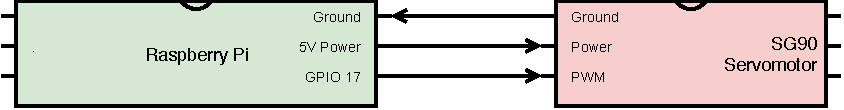
\includegraphics[width=\textwidth]{5-hardwarenutzung/img/servomotor-schaltplan}
        \end{block}
    \end{columns}
\end{frame}
}

%%% Folie
{
\footnotesize

\begin{frame}{Wiederholung: Pulsweitenmodulation}
    \parbox{\linewidth}{
        Die für eine Arbeit zur Verfügung stehende Stromstärke kann nicht nur durch Widerstände
        absolut reduziert werden. Sie kann durch \textbf{Pulsweitenmodulation} (schnelles Ein-
        und Ausschalten) auch im zeitlichen Mittel reduziert werden. Für kurze Zeit fließt dann
        zwar der volle Strom, die Länge der An- und Ausphasen reduziert jedoch die Gesamtstrommenge
        im zeitlichen Verlauf.
    }

    \begin{center}
        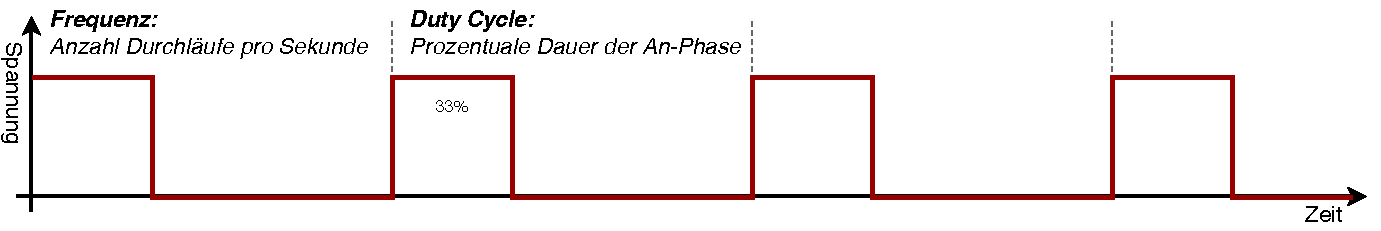
\includegraphics[width=.75\textwidth]{5-hardwarenutzung/img/pwm}
    \end{center}

    \begin{columns}
        \column{.5\textwidth}
        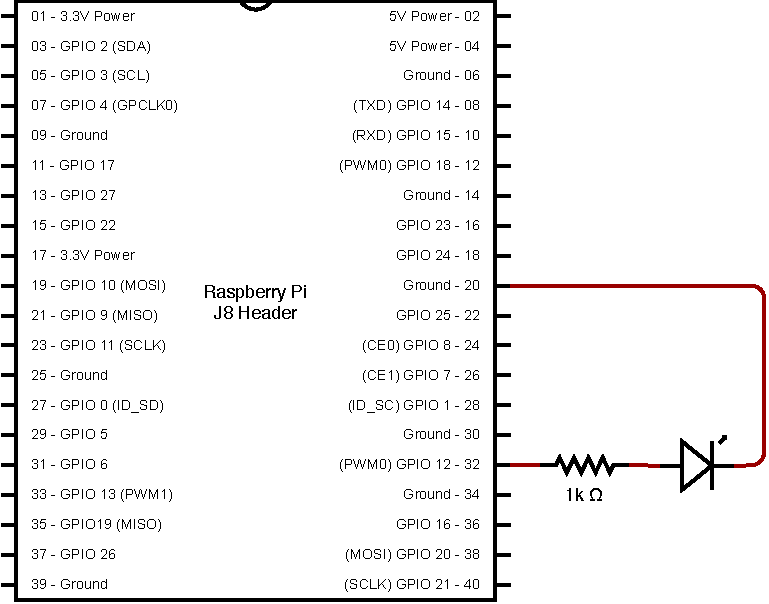
\includegraphics[width=.9\textwidth]{5-hardwarenutzung/img/led_pwm_schaltplan}

        \column{.5\textwidth}
        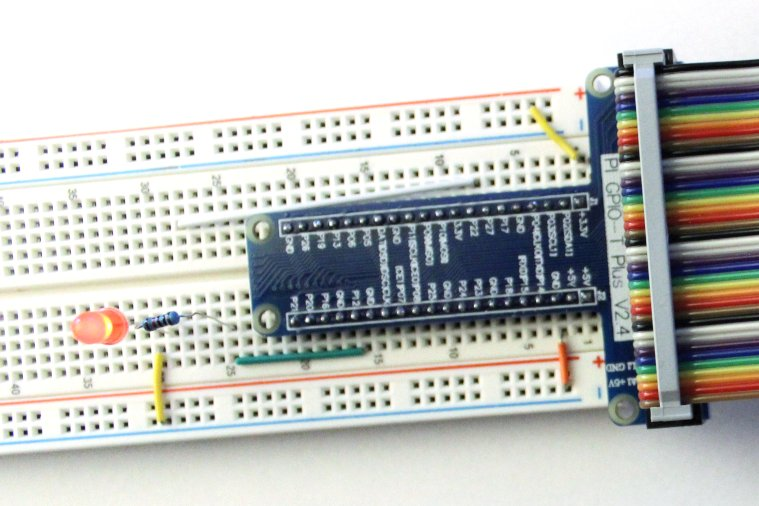
\includegraphics[width=\textwidth]{5-hardwarenutzung/img/led_pwm_foto}
    \end{columns}
\end{frame}
}

%%% Folie
{
\setlength{\leftmargini}{1.2em}
\footnotesize

\begin{frame}[fragile,allowframebreaks]{Programmierung in Python}
    \begin{block}{Initialisieren und Zurücksetzen der GPIO-Pins}
        \begin{lstlisting}[style=MethodenListe, gobble=12]
            import RPi.GPIO as GPIO
        \end{lstlisting}
        Raspberry Pi GPIO-Modul importieren
        \medskip

        \begin{lstlisting}[style=MethodenListe, gobble=12]
            GPIO.setup(10, GPIO.OUT)
        \end{lstlisting}
        GPIO\,10 als Ausgang konfigurieren
        \medskip

        \begin{lstlisting}[style=MethodenListe, gobble=12]
            GPIO.setup(11, GPIO.IN)
        \end{lstlisting}
        GPIO\,11 als Eingang konfigurieren
        \medskip

        \begin{lstlisting}[style=MethodenListe, gobble=12]
            GPIO.setup(12, GPIO.IN, pull_up_down=GPIO.PUD_DOWN)
        \end{lstlisting}
        GPIO\,12 als Eingang mit internem Pull Down konfigurieren
        \medskip

        \begin{lstlisting}[style=MethodenListe, gobble=12]
            GPIO.setup(13, GPIO.IN, pull_up_down=GPIO.PUD_UP)
        \end{lstlisting}
        GPIO\,13 als Eingang mit internem Pull Up konfigurieren
        \medskip

        \begin{lstlisting}[style=MethodenListe, gobble=12]
            GPIO.cleanup()
        \end{lstlisting}
        Alle GPIO-Pins auf eine sichere Standardkonfiguration zurücksetzen
        \medskip
    \end{block}

    \framebreak

    \begin{block}{Lesen und Schreiben einzelner Pins}
        \begin{lstlisting}[style=MethodenListe, gobble=12]
            value = GPIO.input(14)
        \end{lstlisting}
        Aktuellen Zustands von GPIO\,14 (True oder False) lesen
        \medskip

        \begin{lstlisting}[style=MethodenListe, gobble=12]
            GPIO.output(15, True)
        \end{lstlisting}
        GPIO\,15 auf High bzw. 3,3\,V Spannung setzen
        \medskip

        \begin{lstlisting}[style=MethodenListe, gobble=12]
            GPIO.output(16, False)
        \end{lstlisting}
        GPIO\,16 auf Low bzw. 0\,V Spannung setzen
        \medskip
    \end{block}

    \begin{block}{Reagieren auf Interrupts}
        \begin{lstlisting}[style=MethodenListe, gobble=12]
            GPIO.add_event_detect(17, GPIO.RISING, mein_cb)
        \end{lstlisting}
        Callback-Funktion für steigende Flanken auf GPIO\,17 registrieren
        \medskip

        \begin{lstlisting}[style=MethodenListe, gobble=12]
            GPIO.add_event_detect(18, GPIO.FALLING, mein_cb)
        \end{lstlisting}
        Callback-Funktion für fallende Flanken auf GPIO\,18 registrieren
        \medskip
    \end{block}

    \framebreak

    {
        \begin{lstlisting}[style=MethodenListe, gobble=12]
            GPIO.add_event_detect(19, GPIO.BOTH, mein_cb)
        \end{lstlisting}
        Callback-Funktion für jede Änderung von GPIO\,19 registrieren
        \medskip

        \begin{lstlisting}[style=MethodenListe, gobble=12]
            GPIO.add_event_detect(20, GPIO.BOTH, mein_cb, bouncetime=50)
        \end{lstlisting}
        Callback-Funktion für GPIO\,20 mit einer Entprellung von 50\,ms registrieren
        \medskip
    }

    \begin{block}{Pulsweitenmodulation}
        \begin{lstlisting}[style=MethodenListe, gobble=12]
            pwm = GPIO.PWM(21, 100)
        \end{lstlisting}
        Pulsweitenmodulation von GPIO\,21 vorbereiten
        \medskip

        \begin{lstlisting}[style=MethodenListe, gobble=12]
            pwm.start(50)
        \end{lstlisting}
        Pulsweitenmodulation von GPIO\,21 mit 50\,\% Lastzyklus starten
        \medskip

        \begin{lstlisting}[style=MethodenListe, gobble=12]
            pwm.changeDutyCycle(75)
        \end{lstlisting}
        Lastzyklus der Pulsweitenmodulation von GPIO\,21 auf 75\,\% ändern
        \medskip

        \begin{lstlisting}[style=MethodenListe, gobble=12]
            pwm.stop()
        \end{lstlisting}
        Pulsweitenmodulation von GPIO\,21 stoppen
        \medskip
    \end{block}
\end{frame}
}

%%% Folie
\begin{frame}{Quellcodes}
    Siehe Moodle oder \\
    {
        \small
        \url{https://github.com/DennisSchulmeister/dhbwka-wwi-iottech-quellcodes}
    }

    \smallskip
    \setlength{\fboxsep}{0em}
    \fbox{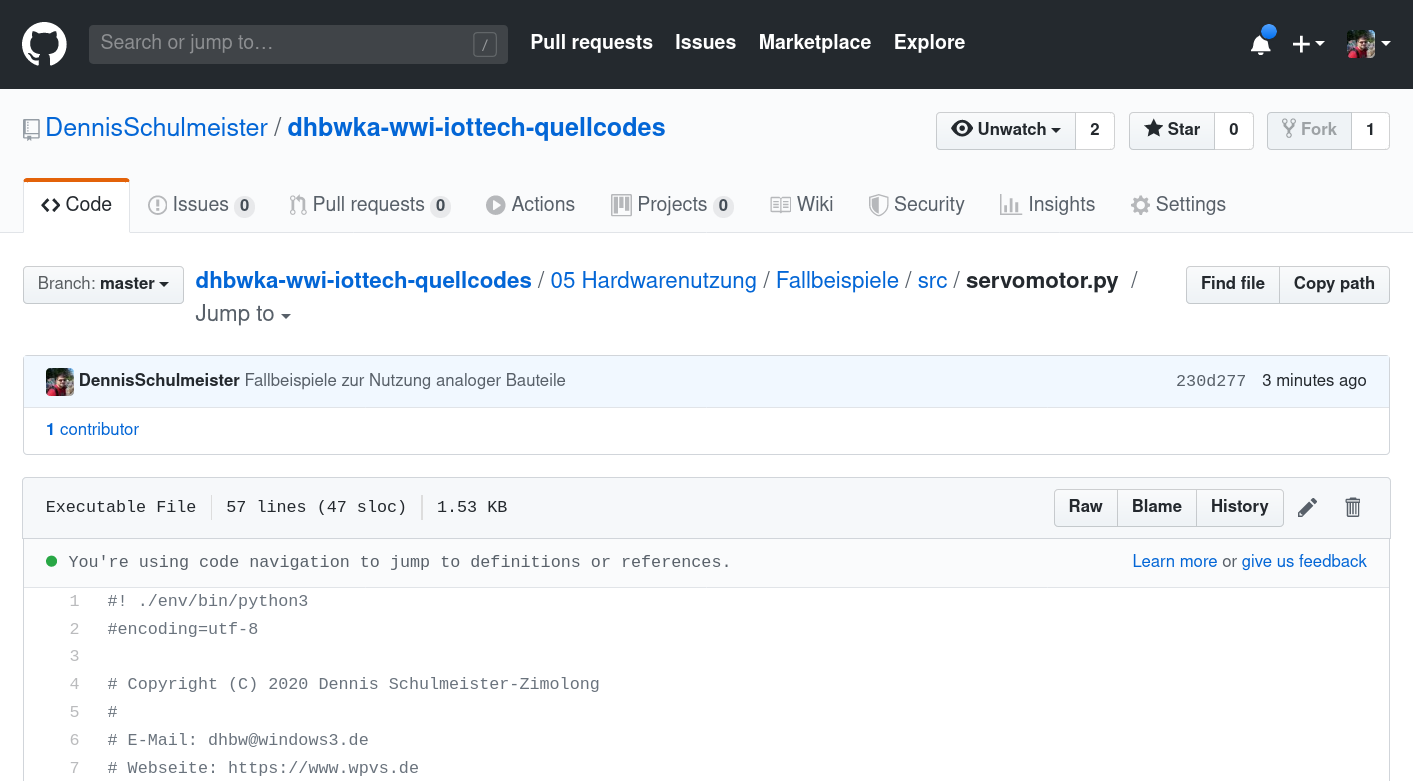
\includegraphics[width=\textwidth]{5-hardwarenutzung/img/github-servomotor}}
\end{frame}

%-------------------------------------------------------------------------------
\section{Serielle Kommunikation}
%-------------------------------------------------------------------------------

%%% Folie
\begin{frame}{Einsatzgebiete serieller Schnittstellen}
    \begin{block}{Speziell auf dem Raspberry Pi}
        \begin{itemize}
            \item Anbindung von Sensoren und Aktoren mit digitaler Schnittstelle
            \item Anbindung analoger Sensoren via seriellem A/D-Konverter
        \end{itemize}
    \end{block}

    \begin{block}{Zusätzlich in eingebetteten Systemen}
        \begin{itemize}
            \item Kommunikation zwischen den einzelnen Subsystemen
            \item Datenaustausch mit anderen eingebetteten Systemen
            \item Datenaustausch mit einem Host-Computer (USB-to-Serial)
        \end{itemize}
    \end{block}

    \bigskip

    \begin{columns}
        \column{.33\textwidth}
        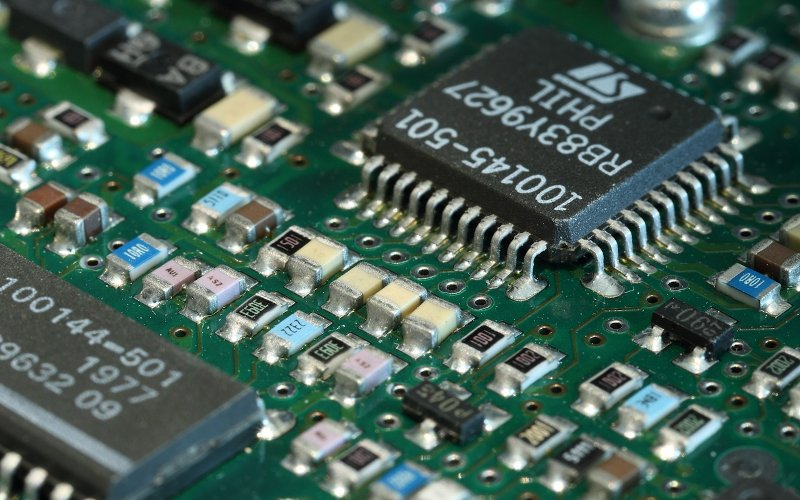
\includegraphics[width=\textwidth]{5-hardwarenutzung/img/seriell_einsatz1}

        \column{.33\textwidth}
        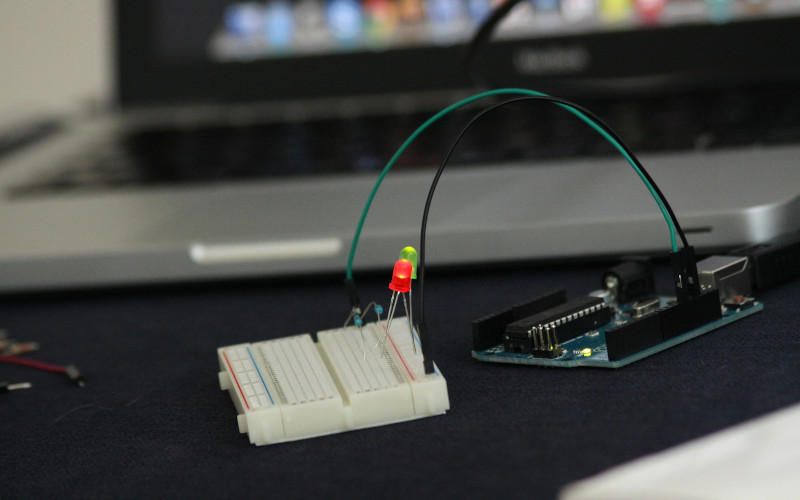
\includegraphics[width=\textwidth]{5-hardwarenutzung/img/seriell_einsatz2}

        \column{.33\textwidth}
        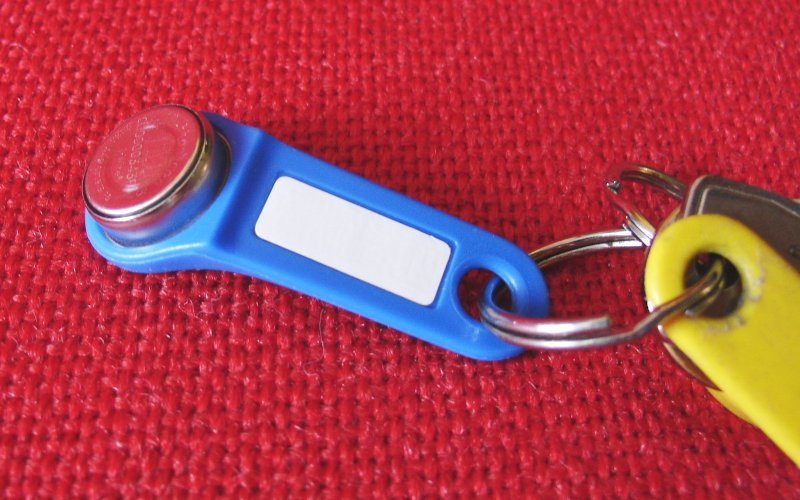
\includegraphics[width=\textwidth]{5-hardwarenutzung/img/seriell_einsatz3}
    \end{columns}
\end{frame}

%%% Folie
{
\footnotesize

\begin{frame}{Funktionsweise der seriellen Datenübertragung}
    \begin{columns}
        \column{\dimexpr\paperwidth-28pt}
        \parbox{\textwidth}{
            Serielle Schnittstellen übertragen digitale Daten durch schnelles Umschalten
            der Logikpegel einer einzigen Datenleitung. Die Schnittstellenart gibt dabei
            vor, wie die Logikpegel in elektrische Signale umgewandelt werden, welche
            Geschwindigkeiten zulässig sind und wie sich Sender und Empfänger synchronisieren.

            \medskip
            \begin{itemize}
                \item \textbf{Synchron:}
                Synchronisation über ein zusätzliches Taktsignal (Serial Clock)

                \item \textbf{Asynchron:}
                Synchronisation über Synchronisationsbits im Datensignal
            \end{itemize}
        }

        \medskip
        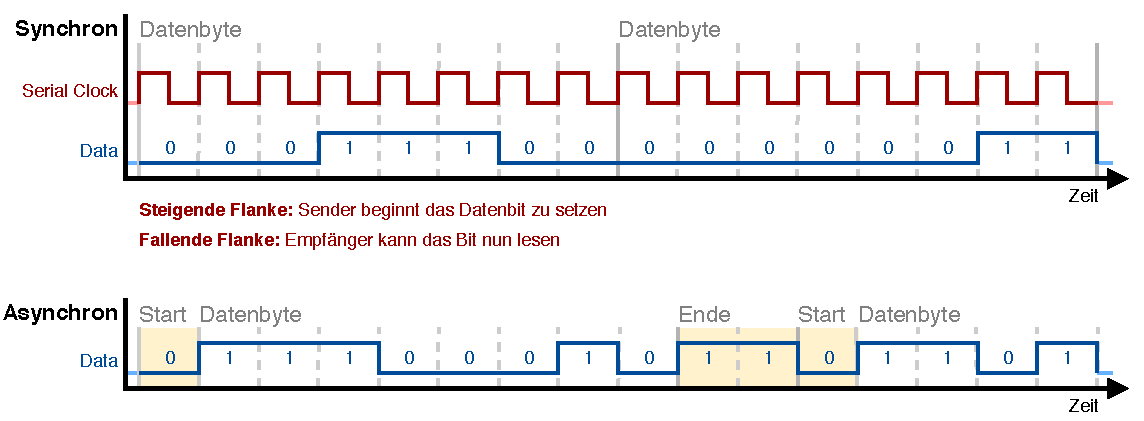
\includegraphics[width=\textwidth]{5-hardwarenutzung/img/seriell_arten}
    \end{columns}
\end{frame}
}

%%% Folie
{
\scriptsize
\renewcommand{\arraystretch}{1.4}
\setlength{\tabcolsep}{0.5em}

\begin{frame}{Übersicht gängiger serieller Schnittstellen}
    \begin{columns}
        \column{\dimexpr\paperwidth-28pt}
        \begin{tabular}{p{.16\textwidth} p{.25\textwidth} p{.25\textwidth} p{.25\textwidth}}
            &
            \textbf{UART} &
            \textbf{I²C} &
            \textbf{SPI} \\
            \hline

            \textbf{Veröffentlichung} &
            1964 & % UART
            1982 & % I²C
            1987 \\ % SPI

            \textbf{Einsatzgebiet} &
            Beliebiger Datenaustausch & % UART
            Anbindung geräteinterner Subsysteme, Sensoren, Aktoren & % I²C
            Anbindung geräteinterner Subsysteme, Sensoren, Aktoren \\ % SPI

            \textbf{Synchronisation} &
            Asynchron & % UART
            Synchron & % I²C
            Synchron \\ % SPI

            \textbf{Geschwindigkeit} &
            50\,Bit/s -- 3\,MBit/s & % UART
            0,1\,MBit/s -- 5\,MBit/s & % I²C
            Typischerweise bis zu 20\,MBit/s \\ % SPI

            \textbf{Topologie} &
            Punkt-zu-Punkt & % UART
            Bus mit einem Master & % I²C
            Sternförmig \\ % SPI

            \textbf{Übertragungsart} &
            Full Duplex & % UART
            Half Duplex & % I²C
            Full Duplex \\ % SPI

            \textbf{Leitungslänge} &
            Typischerweise bis zu 15\,m & % UART
            Typischerweise wenige cm & % I²C
            Typischerweise wenige cm \\ % SPI

            \textbf{Adressierung} &
            Keine & % UART
            Device ID & % I²C
            Zusätzliche Signalleitungen \\ % SPI

            \\

            &
            \textbf{CAN} &
            \textbf{USB} &
            \textbf{MIDI} \\
            \hline

            \textbf{Veröffentlichung} &
            1983 & % CAN
            1996 & % USB
            1986 \\ % MIDI

            \textbf{Einsatzgebiet} &
            Datenaustausch in sicherheitskritischen Bereichen wie Automobiltechnik oder Raumfahrt & % CAN
            Anbindung externer Peripheriegeräte & % USB
            Echtzeitsteuerung von Synthesizern, Tonstudio- und Veranstaltungstechnik \\ % MIDI

            \textbf{Synchronisation} &
            Asynchron & % CAN
            Asynchron & % USB
            Asynchron \\ % MIDI

            \textbf{Geschwindigkeit} &
            125\,kBit/s -- 1\,MBit/s & % CAN
            0,15\,MB/s -- 1,8\,GB/s & % USB
            31.250\,Bit/s \\ % MIDI

            \textbf{Topologie} &
            Bus mit mehreren Mastern & % CAN
            Baum mit mehreren Controllern & % USB
            Bus mit einem Sender \\ % MIDI

            \textbf{Übertragungsart} &
            Half Duplex & % CAN
            Full Dublex & % USB
            Unidirektional \\ % MIDI

            \textbf{Leitungslänge} &
            Typischerweise bis zu 40\,m & % CAN
            Bis zu 5\,m & % USB
            Bis zu 15\,m \\ % MIDI

            \textbf{Adressierung} &
            Keine & % CAN
            Bus und Device ID & % USB
            Keine \\ % MIDI
        \end{tabular}
    \end{columns}
\end{frame}
}

%%% Folie
\begin{frame}{Verdrahtung von SPI und I²C}
    \begin{block}{Serial Peripherial Interface (SPI)}
        \smallskip
        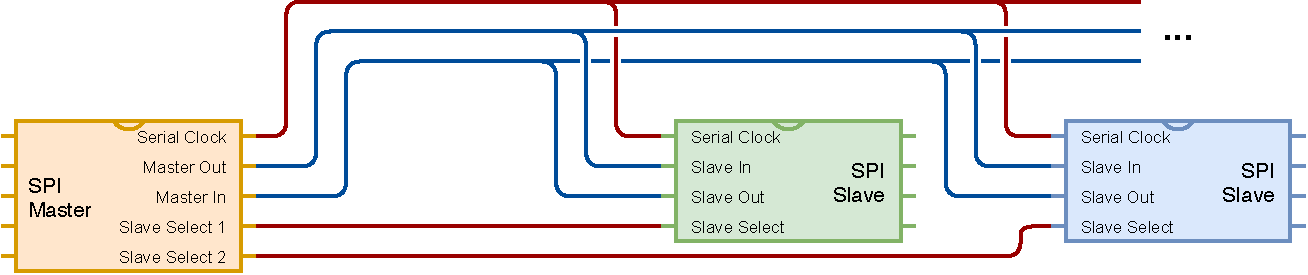
\includegraphics[width=.8\textwidth]{5-hardwarenutzung/img/seriell_spi_schaltplan}
        \smallskip
        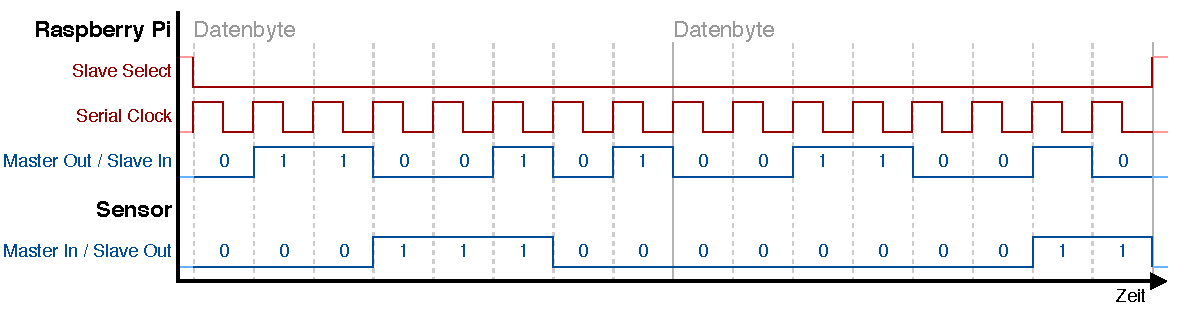
\includegraphics[width=.9\textwidth]{5-hardwarenutzung/img/seriell_spi_timing}
    \end{block}

    \begin{block}{Inter-Integrated Circuit (I²C)}
        \smallskip
        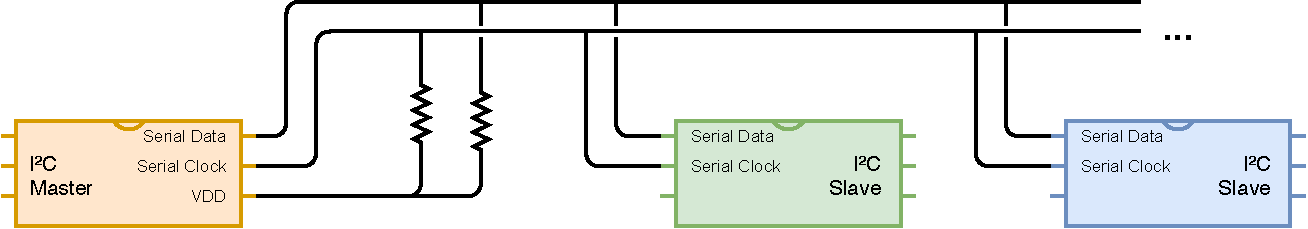
\includegraphics[width=.8\textwidth]{5-hardwarenutzung/img/seriell_i2c_schaltplan}
    \end{block}
\end{frame}

%%% Folie
{
\small

\begin{frame}{Fallbeispiel: Lautstärkenmessung via A/D-Konverter}
    \begin{columns}[onlytextwidth]
        \column{.49\textwidth}
        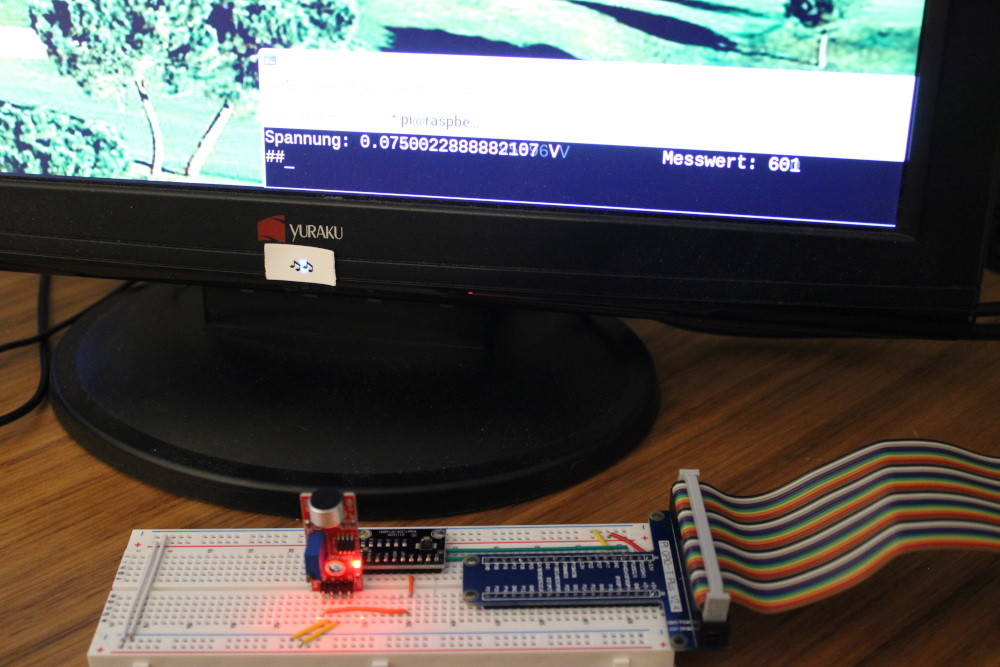
\includegraphics[width=\textwidth]{5-hardwarenutzung/img/lautstaerke-foto1}

        \column{.49\textwidth}
        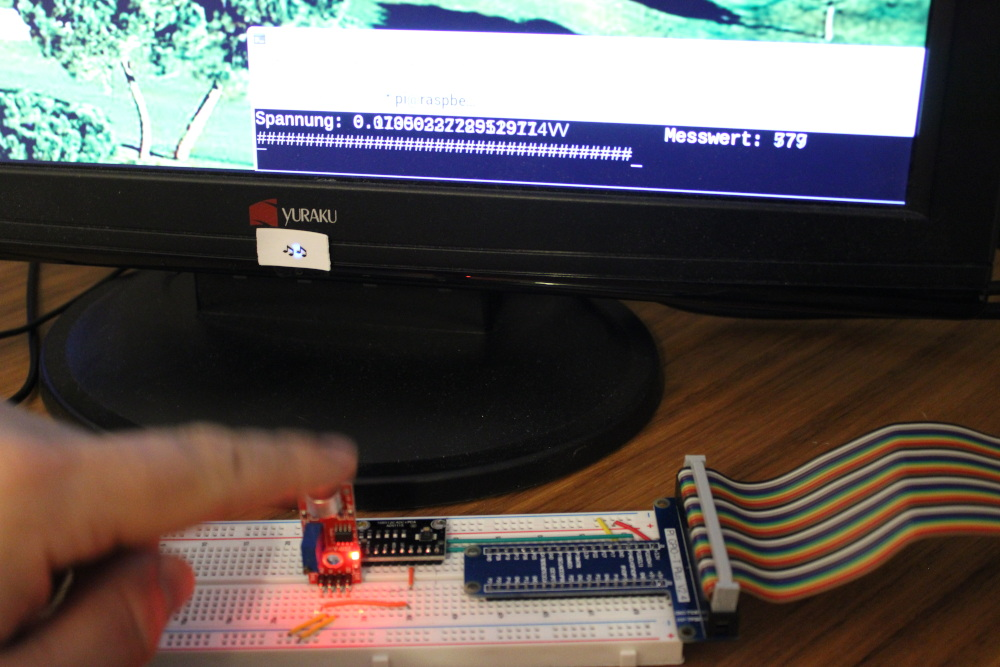
\includegraphics[width=\textwidth]{5-hardwarenutzung/img/lautstaerke-foto2}
    \end{columns}

    \bigskip

    \begin{columns}[onlytextwidth]
        \column{.49\textwidth}
        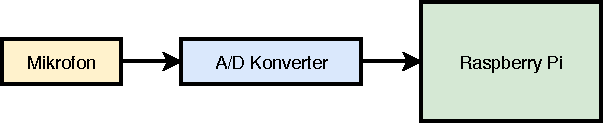
\includegraphics[width=\textwidth]{5-hardwarenutzung/img/lautstaerke-skizze}

        \column{.49\textwidth}
        \parbox{\textwidth}{
            Messung der Umgebungslautstärke mit einem Mikrofon an einem via I²C angebundenen A/D-Konverter.
        }
    \end{columns}

    \bigskip
    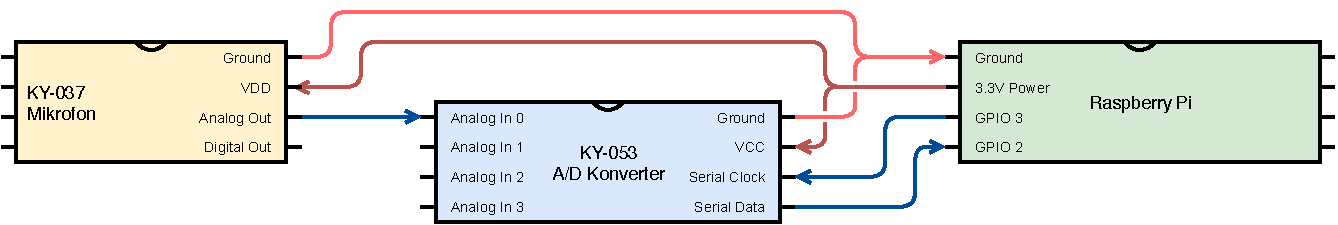
\includegraphics[width=\textwidth]{5-hardwarenutzung/img/lautstaerke-schaltplan}
\end{frame}
}

%~ %%% Folie
%~ \begin{frame}{Fallbeispiel: Datenaustausch mit einem Arduino}
    %~ TODO
%~ \end{frame}

%%% Folie
{
\setlength{\leftmargini}{1.2em}
\footnotesize

\begin{frame}[fragile, allowframebreaks]{Programmierung in Python}
    \begin{block}{Serielle Kommunikation via I²C}
        \begin{lstlisting}[style=MethodenListeKlein, gobble=12]
            import board, busio
            from adafruit_bus_device.i2c_device import I2CDevice
        \end{lstlisting}
        Benötigte Module importieren
        \smallskip

        \begin{lstlisting}[style=MethodenListeKlein, gobble=12]
            i2c_bus = busio.I2C(board.SCL, board.SDA)
            device = I2CDevice(i2c_bus, 0x70)
            device.open()
        \end{lstlisting}
        I²C-Bus und Device mit der Id \texttt{0x70} öffnen
        \smallskip

        \begin{lstlisting}[style=MethodenListeKlein, gobble=12]
            bytes_read = bytearray(4)
            device.readinto(bytes_red)
        \end{lstlisting}
        Vier Bytes vom eben geöffneten Device empfangen
        \smallskip

        \begin{lstlisting}[style=MethodenListeKlein, gobble=12]
            device.write("Hallo, Welt".encode("latin-1"))
        \end{lstlisting}
        Einen String an das eben geöffnete Device senden
        \smallskip

        \begin{lstlisting}[style=MethodenListeKlein, gobble=12]
            device.close()
            i2c_bus.close()
        \end{lstlisting}
        Device und I²C-Bus wieder schließen
        \smallskip
    \end{block}

    \framebreak

    \begin{block}{Serielle Kommunikation via SPI}
        \begin{lstlisting}[style=MethodenListeKlein, gobble=12]
            import board, busio, digitalio
            from adafruit_bus_device.spi_device import SPIDevice
        \end{lstlisting}
        Benötigte Module importieren
        \smallskip

        \begin{lstlisting}[style=MethodenListeKlein, gobble=12]
            spi_bus = busio.SPI(board.SCK, board.MOSI, board.MISO)
            cs = digitalio.DigitalInOut(board.D10)
            device = SPIDevice(spi_bus, cs)
            device.open()
        \end{lstlisting}
        SPI-Bus und Device mit GPIO 10 als Slave Select Leitng öffnen
        \smallskip

        \begin{lstlisting}[style=MethodenListeKlein, gobble=12]
            bytes_read = bytearray(4)
            device.readinto(bytes_red)
        \end{lstlisting}
        Vier Bytes vom eben geöffneten Device empfangen
        \smallskip

        \begin{lstlisting}[style=MethodenListeKlein, gobble=12]
            device.write("Hallo, Welt".encode("latin-1"))
        \end{lstlisting}
        Einen String an das eben geöffnete Device senden
        \smallskip

        \begin{lstlisting}[style=MethodenListeKlein, gobble=12]
            device.close()
            spi_bus.close()
        \end{lstlisting}
        Device und SPI-Bus wieder schließen
        \smallskip
    \end{block}

    \framebreak

    \begin{block}{Serielle Kommunikation via UART}
        \begin{lstlisting}[style=MethodenListeKlein, gobble=12]
            import board, busio
        \end{lstlisting}
        Benötigte Module importieren
        \smallskip

        \begin{lstlisting}[style=MethodenListeKlein, gobble=12]
            uart = busio.UART(board.TX, board.RX, baudrate=9600)
        \end{lstlisting}
        UART-Device mit den Standard-Pins zum Senden und Empfangen und einer Baudrate von 9.600 Bit/s öffnen.
        Ggf. müssen noch weitere Parameter mitgegeben werden, um das richtige Übertragungsformat auszuwählen.
        \smallskip

        \begin{lstlisting}[style=MethodenListeKlein, gobble=12]
            data = uart.read(32)
        \end{lstlisting}
        Bis zu 32 Byte empfangen
        \smallskip

        \begin{lstlisting}[style=MethodenListeKlein, gobble=12]
            line = uart.readline()
        \end{lstlisting}
        Daten bis zum nächsten Zeilenende empfangen
        \smallskip

        \begin{lstlisting}[style=MethodenListeKlein, gobble=12]
            uart.write("Hallo, Welt".encode("latin-1"))
        \end{lstlisting}
        Einen String senden
        \smallskip

        \begin{lstlisting}[style=MethodenListeKlein, gobble=12]
            uart.deinit()
        \end{lstlisting}
        UART-Device wieder schließen
        \smallskip
    \end{block}

    \framebreak

    \begin{alertblock}{Wichtiger Hinweis}
        \smallskip
        \parbox{\textwidth}{
            Für viele Sensoren und Aktoren gibt es spezielle Python-Module, welche die
            Low Level Details der seriellen Kommunikation weg abstrahieren. Bevor man
            also ein Device via I²C oder SPI direkt anspricht, sollte man erst die
            Dokumentation und das Internet konsultieren, ob es nicht eine einfachere
            Möglichkeit der Programmierung gibt.
        }

        \bigskip
        \textbf{Beispiel: Nutzung des A/D-Konverters}

        \begin{lstlisting}[style=MethodenListeKlein, gobble=12]
            import time, busio
            import adafruit_ads1x15.ads1115 as ADC
            from adafruit_ads1x15.analog_in import AnalogIn

            # A/D-Konverter initialisieren, GPIO 3 = Clock, GPIO 2 = Data
            i2c_bus = busio.I2C(3, 2)
            ad_converter = ADC.ADS1115(i2c_bus)
            adc_channel0 = AnalogIn(ad_converter, ADC.P0)

            # Wert messen
            voltage = adc_channel0.voltage
            value = adc_channel0.value

            # Device schließen
            i2c_bus.deinit()
        \end{lstlisting}
    \end{alertblock}
\end{frame}
}

\begin{frame}{Quellcodes}
    Siehe Moodle oder \\
    {
        \small
        \url{https://github.com/DennisSchulmeister/dhbwka-wwi-iottech-quellcodes}
    }

    \smallskip
    \setlength{\fboxsep}{0em}
    \fbox{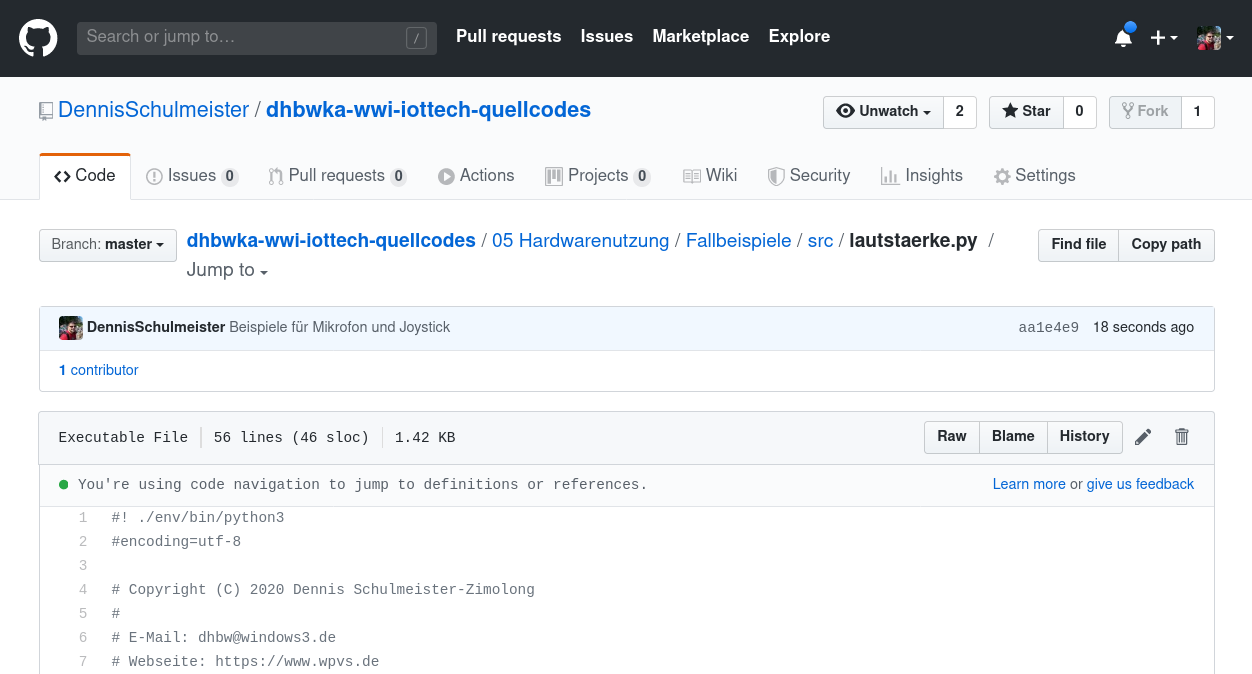
\includegraphics[width=\textwidth]{5-hardwarenutzung/img/github-lautstaerke}}
\end{frame}
